\subsubsection{Classification de documents}

L'un des domaines dans lequel l'intelligence artificielle excelle et s'améliore rapidement de nos jours est la classification, que ce soit des documents, images, textes, mails, etc.

Dans une GED, avec une architecture et une organisation précise prédéfinie, il peut être intéressant d'utiliser un système permettant de classer les documents importés au bon endroit au sein de la structure sans que l'utilisateur n'ait besoin d'intervenir.
Afin de fonctionner correctement, un tel système nécessite de nombreuses données d'entraînement.
C'est grâce à ces dernières qu'il pourra apprendre à classifier correctement les documents au sein de l'architecture.
Un tel système ne peut donc être mis en place que sur une GED ayant été classée manuellement depuis un certain temps, afin d'avoir plusieurs exemplaires de chaque type de documents déjà classés au sein de l'architecture.

Il existe de nombreux concepts d'intelligence artificielle permettant de classifier des fichiers.
Les plus poussés sont actuellement les réseaux de neurones à convolution qui permettent de classifier des images avec des taux d'erreur extrêmement bas.
Cependant, nous voulons ici classifier des documents et nous allons voir que nous pouvons utiliser des concepts beaucoup plus basiques et requérant bien moins de puissance de calcul pour atteindre un résultat satisfaisant.

\paragraph*{Préparation des documents}
~\\

Pour classer un document, les êtres humains sont capables de repérer quasiment instantanément les détails permettant d'en identifier la nature exacte, que ce soit par la lecture de certains mots clés ou par le repérage d'un logo par exemple.
L'objectif ici est de trouver un concept d'intelligence artificielle qui soit capable de faire la même chose.

Il y a deux possibilités majeures sur la manière dont le système peut traiter des documents.
\\
\begin{itemize}
    \item[\tiny$\bullet$] La première serait de considérer les documents comme des images.
    Le principal avantage serait que si des documents sont principalement discernables de par leurs caractéristiques graphiques plus que de par leur contenu, le système serait capable de les classifier sans difficulté.
    Cependant, le cas inverse se présente également et comme nous traitons ici des documents généralement administratifs, il est plus courant que ces documents aient une charte graphique semblable et se discernent principalement de par leur contenu.
    En plus de cela, les documents n'ont pas toujours le même nombre de pages. Or il est très préférable que toutes les images à classifier aient les mêmes dimensions pour que ce genre de systèmes fonctionnent correctement.
    
    \item[\tiny$\bullet$] La seconde possibilité est de préalablement extraire le texte des documents afin de pouvoir se baser sur le contenu de ceux-ci pour les classer.
    Pour extraire le texte brut d'un document il existe de nombreuses méthodes d'OCR, en français reconnaissance optique de caractères, qui sont robustes et utilisables sur des pdf complets en une simple ligne de code~;~il n'est donc pas intéressant de les décrire plus que cela.
    Avant de donner tout le texte d'un document à un système de classification, il est cependant nécessaire d'effectuer des traitements permettant d'en extraire des <<~features~>>, <<~caractéristiques~>> en français.
    C'est sur ces caractéristiques que le système pourra se baser afin de classer les documents.
    Une démarche intéressante serait par exemple d'utiliser la méthode de pondération TF-IDF (term frequency-inverse document frequency).
    Celle-ci est très utilisée en fouille de textes, car elle permet de mesurer l'importance de chaque terme employé dans un texte.
    Avec cette méthode on pourrait, par exemple, extraire les cinq termes les plus importants dans le document et utiliser uniquement ces cinq termes afin de classer ce dernier.
\end{itemize}
~\\

Dans notre cas, la meilleure solution serait sans doute d'utiliser la seconde méthode, consistant en l'extraction des principales caractéristiques directement depuis le texte de chaque document.
Avec cette méthode on peut donc générer une base de données reliant les termes les plus importants avec chaque document dont ils sont extraits.
Ainsi, nous posséderions une base de données avec tous les documents déjà présents dans la GED, ces données serviraient de données d'entraînement au système de classification.
Une fois le système entraîné, lorsqu'un nouveau document sera importé, il suffira d'en extraire les caractéristiques et de les envoyer dans le système pour que le document soit classé automatiquement.

\paragraph*{Algorithmes de classification}
~\\

Une fois les données prêtent, nous pouvons analyser les documents en comparant le nombre de termes en communs parmi leurs caractéristiques extraites.
C'est pour effectuer cette comparaison que l'algorithme de classification va entrer en jeu.
Sachant que les caractéristiques extraites ne seront pas très nombreuses on peut utiliser des classifieurs linéaires relativement basiques, tels que les SVM (<<~support vector machine~>> traduit par <<~machine à vecteurs de support~>>),  la classification naïve bayésienne, ou même la méthode des $k$ plus proches voisins.

Les trois méthodes précédemment citées sont des concepts de base de l'intelligence artificielle qui sont enseignés en tant qu'introduction dans beaucoup de cours, portants sur l'intelligence artificielle.
Cependant, cela ne signifie pas qu'ils sont inutiles ou inefficients~;~ils sont au contraire, simple à développer et à appliquer, et peuvent être utilisés lorsque la situation s'y prête.
Comme déjà précisé, nous nous basons sur un nombre de caractéristiques très limité pour cette classification.
Ces classifieurs sont donc adaptés à notre cas de figure avec des avantages et inconvénients pour chacun d'entre eux.
\\
\begin{itemize}
    \item[\tiny$\bullet$] Le principe des machines à vecteurs de support (séparateurs à vaste marge) est de placer des frontières entre les catégories.
    On peut en visualiser le fonctionnement facilement si on prend un exemple simple de classification ne contenant que deux classes.
    Considérons les données suivantes, dans lesquelles les deux classes sont <<~ronds~>> et <<~triangles~>> et la donnée que l'on veut classer dans une de ces dernières est le carré rouge.
    
    \FloatBarrier
    \begin{figure}[h!]
        \begin{minipage}[c]{0.5\textwidth}
            \begin{center}
                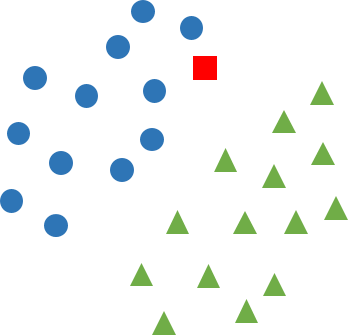
\includegraphics[width = 0.35\textwidth]{svm_1}
            \end{center}
        \end{minipage}\hfill
        \begin{minipage}[c]{0.5\textwidth}
            \caption{Problème de classification en deux dimensions}
            \label{figure:svm_1}
        \end{minipage}
    \end{figure}
    \FloatBarrier
    
    En tant qu'être humain, il est trivial de déterminer que le carré devrait être classé avec les ronds, au vu de l'organisation présente.
    C'est cependant nettement plus complexe pour une machine.
    Le but du SVM va être de déterminer une droite <<~frontière~>> qui permette de séparer les données en deux classes.
    Le SVM choisit une frontière qui maximise la marge, c'est-à-dire qu'elle est le plus éloignée possible des deux classes.
    Cela permettra de classer avec plus de précision les futures données inconnues.
    
    Par exemple, dans la figure ci-dessous on voit deux frontières noires en pointillés qui permettent de classifier correctement les données d'entraînement.
    En revanche elles ne maximisent pas la marge entre les deux classes, ce qui peut donner lieu à de mauvaises classifications dans le futur.
    La frontière maximisant la marge, qui sera donc déterminée par le SVM, est symbolisée en rouge.

    \FloatBarrier
    \begin{figure}[h!]
        \begin{minipage}[c]{0.5\textwidth}
            \begin{center}
                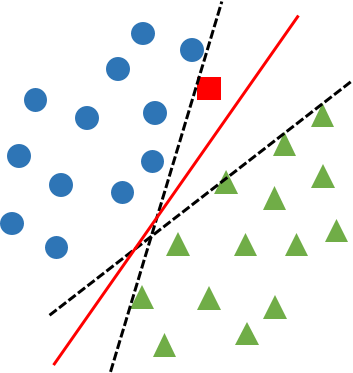
\includegraphics[width = 0.35\textwidth]{svm_2}
            \end{center}
        \end{minipage}\hfill
        \begin{minipage}[c]{0.5\textwidth}
            \caption{Détermination de la frontière maximisant la marge par le SVM}
            \label{figure:svm_2}
        \end{minipage}
    \end{figure}
    \FloatBarrier
    
    Les SVM peuvent classifier des données avec plus de deux dimensions, ils s'appliquent donc correctement à notre cas.
    
    Avant de pouvoir utiliser un SVM pour classer des données il faut déjà que celui-ci soit entraîné.
    Cet entraînement s'effectue grâce aux données déjà présentent au sein de la GED (plus le nombre de classes et de caractéristiques sera élevé et plus le temps et les besoins en puissance de calcul augmenteront).
    Cela signifie que pour entraîner un SVM il faut utiliser une machine assez performante.
    Dans notre cas, le nombre de classes de documents et de caractéristiques utilisées devrait rester assez limité pour qu'une machine récente soit capable de réaliser cette tâche.
    L'avantage est que, une fois l'entraînement du SVM effectué, il peut être utilisé sur un ordinateur extrêmement peu puissant afin de classer de nouvelles données.
    Les utilisateurs de la GED pourront donc utiliser n'importe quel type de matériel.
    ~\\
    
    \item[\tiny$\bullet$] La classification naïve bayésienne est basée sur le théorème de \textsc{Bayes} et utilise des formules de statistiques.
    
    Le théorème de \textsc{Bayes} est le suivant~:~
    $$P(h|d) = \frac{(P(d|h) \cdot P(h))}{P(d)}$$
    Où~:~
    \begin{itemize}
        \item[\tiny$-$] $P(h|d)$, est la probabilité de l'hypothèse $h$ sachant la donnée $d$.
        \item[\tiny$-$] $P(d|h)$, est la probabilité de la donnée $d$ sachant que l'hypothèse $h$ est vraie.
        \item[\tiny$-$] $P(h)$, est la probabilité que l'hypothèse $h$ soit vraie.
        \item[\tiny$-$] $P(d)$, est la probabilité de la donnée $d$.
    \end{itemize}
    Dans notre cas, nous voulons calculer toutes les probabilités du type \textit{P(caractéristique$|$classe de document)}.
    Par exemple, la probabilité \textit{P(livraison$|$bon de livraison)} sera élevée puisque le terme <<~livraison~>> sera une caractéristique forte des documents de classe <<~bon de livraison~>>, tandis que \textit{P(facture$|$bon de livraison)} sera basse.
    
    On calcule ainsi toutes les probabilités d'apparition des caractéristiques pour chaque classe.
    Ensuite lorsque nous voulons classer un nouveau document il suffit d'extraire ses caractéristiques et d'observer les probabilités du type P(classe$|$caractéristique) et la plus haute donnera la classe du document.
    ~\\
    
    \item[\tiny$\bullet$] La méthode des $k$ plus proches voisins est une méthode qui à l'avantage d'être plutôt intuitive et donc simple à comprendre et implémenter.
    Le but est ici de comparer les caractéristiques du nouveau document avec les caractéristiques de tous les documents déjà présents dans la GED.
    Une fois cette comparaison effectuée, le document le plus <<~proche~>> du nouveau est celui qui aura le plus de caractéristiques en commun avec lui.
    Le nouveau document est classé dans la même classe que le voisin le plus proche.
    
    L'explication ci-dessus ne prend en compte qu'un seul voisin le plus proche.
    Cependant pour de meilleures performances il peut être intéressant de sélectionner, par exemple, les cinq voisins les plus proches et attribuer au nouveau document la classe apparaissant le plus souvent parmi ces derniers.
    Le nombre de voisins considérés correspond à la variable $k$.
    Il est préférable de toujours choisir une valeur de $k$ impaire afin de toujours pouvoir déterminer une classe sans souci.
    
    Le principal désavantage de cette méthode est qu'elle ne possède pas de phase d'apprentissage à proprement parler.
    À la place la totalité des échantillons présents dans la base sont parcourus à chaque ajout de nouveau document.
    Cela est fortement contraignant, car plus le nombre de documents présents dans la GED sera grand, plus le processus de classification des nouveaux sera long.
    Cela signifie aussi que les utilisateurs de la GED doivent posséder un ordinateur capable d'une puissance de calcul suffisante pour classer chaque nouveau document.
\end{itemize}
~\\

Pour choisir une méthode de classification parmi les trois proposées ci-dessus, il faut analyser leurs défauts et avantages.
En termes de puissance de calcul nécessaire, le choix se portera sans nul doute sur la classification naïve bayésienne.
Celle-ci nécessite juste le calcul d'un nombre fortement limité de probabilités que n'importe quelle machine peut assumer, la classification des nouvelles données se fait ensuite instantanément.
En revanche, le SVM n'est un choix valable qu'en possession d'une machine permettant son entraînement.
La méthode des $k$ plus proches voisins est, quant à elle, peu envisageable, sachant qu'elle nécessite que tous les utilisateurs possèdent une machine puissante, de plus, son processus de classification est lent.

Afin d'aller plus loin, et d'éventuellement améliorer la précision de la classification, on peut imaginer un système se basant à la fois sur des caractéristiques provenant du texte et d'autres provenant de la charte graphique du document.